\section{General Practices}
\label{imp:general_practices}

Software development is hard and, at times, frustrating. The following
general practices should allow for greater productivity, higher
quality software and less frustration involved in the process of creating it.

\subsection{Documenting Functions}
When writing code, it is valuable to spend time making sure the
code is readable. One way of increasing readability is to provide comments
to non-trivial code samples. Doing this, the programmer will not only
help himself, but also his peers, in later reading and understanding of the code.

When providing comments to top-level functions in C\#, it is
recommended to do so by using XML comments as seen in
\cref{fig:xml_comments_example}. By structuring the comments above a
corresponding top-level function, other software can present nicely
viewable code documentation.

\begin{lstlisting}[caption = {Example of XML-comments on top of C\# function.}, label={fig:xml_comments_example}]
/// <summary>
/// Gets list of unique tracks from JSON
/// </summary>
/// <param name="jsonCode">JSON collection of tracks</param>
/// <returns>List of tracks contained in JSON</returns>
private List<Track> GetTracks(JToken jsonCode) {
\end{lstlisting}


\chapter{Design Patterns}

\alnote{mangler intro tekst}

\section{Model View Viewmodel}

This project is both on the client and on the server structured using
the Model View ViewModel (MVVM) pattern \cite{mvvm}. The core idea in MVVM is to
separate the presentation layer, the view in MVVM, from the model
layer, the model in MVVM. This separation is done by introducing a
ViewModel layer. The ViewModel exposes data from the model to the view
in such a way that the view layer never has any knowledge about the
model layer. This is achieved by databinding elements on the view
layer to model data exposed through the viewmodel.

The benefits of MVVM is that it provides a clean template for
separating the view logic from the business logic and from the data
layer.

This pattern is used mainly because the frameworks used on the client
and server are designed to be structured using this pattern. Other
similar patterns such as Model View Controller (MVC) could
theoretically also have been used, but doing so would go against some
of the principles the frameworks used are based upon.

\section{Singleton Pattern}

The singleton pattern is used whenever there should only ever be one
instance of a class \cite{skeet2013c}. The pattern is often implemented as a static
method on the class, that instantiates the class on the first call,
and on later calls returns the created instance of the class.

This pattern is used in SpotifyDotNet, the libspotify wrapper, used in
this project. Because it is only possible to be logged in one user at
a time, the SpotifyLoggedIn class implements the singleton pattern.

\section{Dependency Injection}

Dependency Injection is a design pattern that helps to reduce coupling
between different components in a software program \cite{injection}. The main idea is
to have components not depend on concrete dependencies but instead
depend on abstractions of dependencies. Doing this, dependencies can
be dynamically changed during runtime as long as their abstractions
match up.

In this project the StructureMap framework\footnote{http://docs.structuremap.net/} is used to reduce
boilerplate and ease the implementation of Dependency
Injection. StructureMap needs to be set up when the application
starts. That is, every dependency abstraction has to be mapped to a
concrete dependency. The dependency abstractions are modelled using
C\# interfaces. An example of an abstraction can be seen in \cref{fig:dep_abstraction}.

\begin{lstlisting}[caption = {Abstraction of a dependency abstraction
    using C\# interfaces. A concrete dependency has to implement the
    methods described in the abstraction.}, label={fig:dep_abstraction}]
public interface IPlaylistService
    {
        Track FindTrack(string trackUri);
        void Add(Track track);
        ConcurrentBagify<Track> Tracks { get; }
        int CalcTScore(Track track);
        Track NextTrack();
    }
\end{lstlisting}

To make use of a dependency in a component, the abstraction of the
dependency just has to be a parameter to the constructor of the
component. The StructureMap framework will then automatically inject
the concrete dependency that was mapped to the abstraction of the
dependency into the component. An example of this can be seen in
\cref{fig:injection}. So by using dependency injection, no component
has ever any knowledge of which concrete dependency it is using. The
component only knows that it depends on an abstraction of a
dependency. This property leads to several benefits, including
modularity of the code. That is, a whole dependency can be swapped for
another dependency as long as they both implement the abstract
dependency model.

\begin{lstlisting}[caption = {Dependency Injection through class
    constructors. IPlaylistService, IUserService and IPlaybackService
    are all abstractions of dependencies.}, label={fig:injection}]
public VoteService(IPlaylistService playlistService, IUserService userService, IPlaybackService playbackService) {
            _playbackService = playbackService;
            _playlistService = playlistService;
            _userService = userService;
        }
\end{lstlisting}


\chapter{Client}

This chapter describes the client side of the solution, and which frameworks are used in this project, in order to design a cross platform mobile application. 

\section{Native Application Development Framework}
\label{par:native_application_development_framework}

Many native application development frameworks exist, including Android SDK, iOS SDK, Windows Phone SDK, Qt, Xamarin.Forms and more. They each have their different characteristics. Android SDK makes it possible to build Android applications. The applications are written in the programming language Java. Similarly you can use iOS SDK to build iOS applications and Windows Phone SDK to build Windows Phone applications using Objective C or Swift, and C\# respectively. Qt is cross platform, so the application written using Qt can run on a variety of systems including Android, iOS and Windows Phone. Qt is written in the programming language C++. Xamarin.Forms is also cross platform and is written in C\#.

With so many good frameworks it is hard to choose one to go with. Fortunately the semester description helps to decide by specifying that all programming should be in C\#. This narrows the possibilities of frameworks down to Xamarin.Forms or limiting the platforms to only Windows Phone devices.

Limiting the application to only Windows Phone devices would drastically limit the amount of devices which could run the application

Xamarin.Forms makes it possible to write an application in C\# and run it on iOS, Android and Windows Phone. The application will look differently on the three platforms, but they will feel native on each of the platforms.

Because Xamarin.Forms enables native applications for all three large mobile platforms, the client application can reach a large user base. The client application is therefore chosen to be written using the Xamarin.Forms framework.
%%% Local Variables:
%%% mode: latex
%%% TeX-master: "../../master"
%%% End:


\chapter{Server}

This chapter describes how the server side functionality of the solution is implemented. It is described how the third party frameworks are used to obtain meta data, and stream the music. Additionally, the steps which were taken to ensure the quality of the solution will be characterised.

\section{White- and Blacklist}
As described in \cref{sec:restrictions} the system should implement a form of restriction though white and black listing. An obvious implementation is to whitelist and blacklist specific tracks in the music catalogue. Making such a filter could be a very tedious process with a very large music catalogue. Somehow easing the process of making restrictions would be beneficial for the administrator, this could be implemented by allowing for creation of coarser restrictions. The coarser restrictions are based on metadata related to the tracks, beside the title; the artist of the track, the genre of the track and some signature tags, like "fast pace" or "electronic". Spotify provides very limited metadata in their database of music, but does include the most significant ones such as, what album the track is on, the artists who made the track, if it is explicit, the length of the track and occasionally the genre and popularity. Further tags and metadata could be provided by a third party database, such as Musicbrainz. An implementation of another provider of metadata, was concluded to be outside of the scope of the project, as metadata is available through Spotify. To avoid that the same track is found across both databases, an International Standard Recording Code (ISRC) is provided from Spotify’s database. This can be used to uniquely identifying a music track across multiple databases \cite{isrc}.

The restrictions are implemented as a list of predicates, that each individual track must meet in order to be added to the playlist. These predicates return boolean value indicating whether a track is allowed e.g. by evaluating the artists of the track, if a blacklisted artist occurs on the track. When the user is searching for a track, it will be marked as not available to explicitly state that the track was indeed found in the music catalogue, but is not allowed to be played at the specific venue. This is done in order to minimize any confusion during the search phase.

\section{Track Duplicates in Music Catalogue}
\label{sec:duplicates}
The same track can appear multiple times in the music catalogue, if multiple versions of the track, with different meta data, exist, e.g. the track \enquote{Dancing Queen} made by ABBA appears on the albums \enquote{ABBA Gold} and \enquote{Arrival}. This is a problem since it could create confusion for the user about which track to vote for.

One solution of this problem is to use additional identifiers of the
meta data associated with a track. Two tracks are most likely
identical if their titles, names of artists, their years of recording and
their recording codes are all equal. Additionally, tiny variations in
the meta data can be allowed. For example, if the difference of the duration of the
two tracks is within 10 seconds, and all the prior mentioned meta data
matches up, the two tracks are probably identical.

\section{Access to Spotify}
\label{sub:Access_to_Spotify}

As it is now established that Spotify is the music catalogue of choice, it is important to think of ways to access their data. As of this paper, two main APIs are available: Spotify Web API and libspotify. They each have their benefits and restrictions.

\subsection{Spotify Web API}
\label{techPlat:music_catalog_web_api}

The Web API is the easiest of the two to work with. It is not needed to login with a Spotify account to use this API, however when the user is authorized, rate limits improve. The API is accessed as a simple REST based interface to nearly all their data. That is, tracks, albums, artists, playlists, user profiles, album art and track previews are all accessible. Notice that this is only metadata about tracks, albums etc. Besides the track previews, no music can be streamed using this API.

So the price of simplicity and ease of use is the limitation of only being allowed to access metadata.

\subsection{Libspotify}
\label{techPlat:music_catalog_libspotify}

Libspotify is a C library written and distributed by Spotify. It is more feature-rich and complex than the Web API. The library can access any data that the official Spotify client can. In fact, the official Spotify client uses libspotify. This implies that both accessing metadata, searching and music streaming is possible. The downside to this more powerful library is the requirement of a Spotify Premium account and the complexity of managing memory and threads.

\subsection{Conclusion}
\label{ssub:music_catalog_conclusion}

Based on the knowledge acquired above it is determined that the web API is best used for retrieving metadata by searching Spotify's data. It is easily integrated in different contexts, as the only requirement is an internet connection.

Libspotify is best used in a context where playback of tracks are needed and the requirement of a Spotify Premium account is no problem.
%%% Local Variables:
%%% mode: latex
%%% TeX-master: "../../master"
%%% End:


This section works with how the structure of the classes are build around Spotify Web API [AND POSSIBLY THE WHOLE PROJECT], and what considerations and approaches that has been taken into consideration, when designing the architecture. 


When using the Web API to search on Spotify, three different items can be found Track, Album and Artist. These three items are all identified by a unique ID from Spotify, which is what is also used as the id for the item in this project. A small problem occurs in the implementation of this search since it is required to specify what item is being searched for. The user, although always eventually looking for a track, does not always find the track directly via the title, but often via the artist by whom it was created or album on which the track is placed. It was therefore chosen that each search requires a specification on what type item that is being searched for. To minimize the requirements for the user, it was decided that the user him or her self, should not specify what item he or she is searching for himself, but rather he or she should write the search string, and get a complete list of the results for all items represented. Therefore it has been implemented, that it is possible, when creating a Search object, to specify from an enum which of the three items or all three are being searched for. When choosing all three, which is what is done for the users searches, three individual searches are created and the results are represented in a complete structure shown in \cref{fig:WebAPIUML}.

\begin{figure}[H] 
\centering 
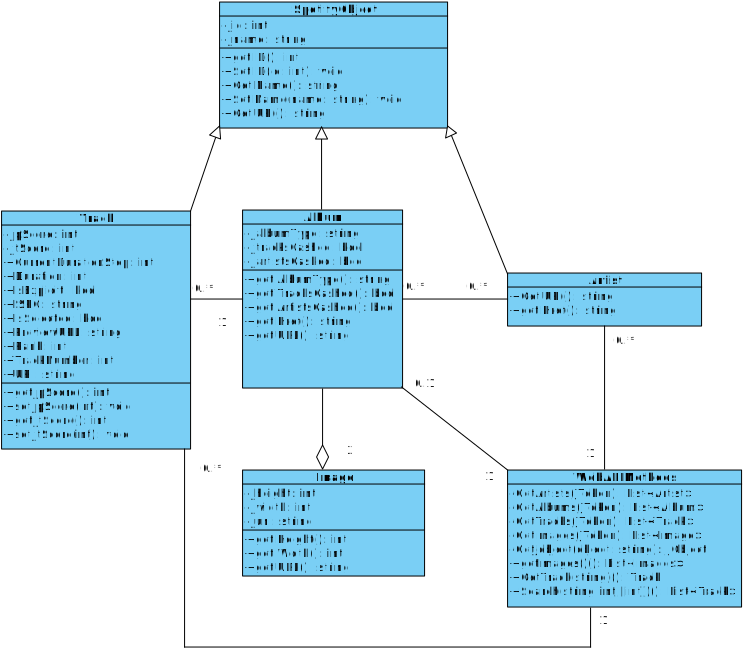
\includegraphics[width=\textwidth]{Images/WebAPIUML.png} 
\caption{A class diagram showing the class structure of the results generated from a search} 
\label{fig:WebAPIUML} 
\end{figure} 


It was decided to have a minimal data download approach when designing the web API. This was done on the bases of the assumption that this API would most likely be the system used for searching for new tracks on the mobile front-end application. Since mobile phones still have limited data access, it is preferable for the user to use as little data as possible. This approach results in that only three searches, one for each item type, are done initially and other requests are not done until other information about the item is needed (this will explained shortly). Furthermore this approach also resulted in all information is stored in the objects locally, and is saved until the search object is removed, and the user hopefully has found his or her track.


As mentioned earlier one search usually searches for all three different item types, track, album and artist, and present these to the user. Not all information about the artists and albums can be gathered from the json code received from these three initial searches. Albums does not have information about it tracks nor its artists initially, and an artist does not have information about its albums. The minimal data approach was therefore combined with another idea, data just in time. This was done since the user normally only wants information from one type of item, and not the two remaining types. It would therefore be undesirable for the user to wait, for all information for every item to be downloaded. This also fits very well with the minimal data approach since this, if the user does not look though all items in the search, minimize the amount of data requested. The information not received from the initial searches, are therefore only requested from Spotify when the get method for the properties on items are called, but to keep faithful to the minimal data approach these information, when first received, are cached to the application and saved in the object structure so that the data does not have to be downloaded again.

As stated in \cref{par:music_catalog_libspotify} the only way to stream tracks off Spotify is using the C library libspotify. Being written as a C library, one has to take care of managing memory allocation correctly in order to avoid runtime exceptions while using libspotify. 

To make it harder to cause these runtime errors and to ease interoperability in the C\# environment, a C\# library can be written that abstracts the error prone elements of C programs away. The C\# library \enquote{SpotifyDotNet} developed for use in the software described in this paper, does just that.

\subsubsection{Abstracting Low-level C Concepts Away}
\label{ssub:abstracting_low_level_c_concepts_away}

The goal of the SpofityDotNet library is to minimize runtime exceptions caused by memory related errors. To do this, the error prone unmanaged C code has to be accessed as secure managed C\# code.

SpotifyDotNet uses existing bindings, hosted on \url{http://libspotifydotnet.codeplex.com/} \sinote{Hvad med licens?}, to interface with libspotify from C\#. As an example let's look at the login function from libspotify. See \cref{fig:loginC}. The corresponding binding can be seen in \cref{fig:loginCsharp}. As can be seen, a C pointer maps directly to an IntPtr struct in C\#. \enquote{const char*} becomes a common string object in C\#. A C bool is simply a C\# bool.

\begin{lstlisting}[caption = {Libspotify login function prototype - C}, label = {fig:loginC}]
sp_error sp_session_login ( sp_session *session,
                            const char *username,
                            const char *password,
                            bool remember_me,
                            const char *blob
                          )
\end{lstlisting}

\begin{lstlisting}[caption = {Login method using a external implementation from libspotify.dll - C\#}, label={fig:loginCsharp}]
public static extern sp_error sp_session_login ( IntPtr sessionPtr, 
                                                 string username, 
                                                 string password, 
                                                 bool rememberMe, 
                                                 string blob 
                                               )
\end{lstlisting}

However this is not abstracted enough. To the user of the library, no pointers should be visible. This is solved by encapsulating state and data inside the Spotify class. This class is the entry point to using libspotify in C\#. See \cref{fig:spotifydotnet_class} for a complete class diagrams. The main operation on the class is the Login method. This method is asynchronous so will return execution to the caller right away. When login has occurred, either OnLogInSuccess or OnLogInError callbacks will be called. These are implemented as C\# events, making it possible for multiple subscribers to listen to this callback. The OnLogInSuccess event sends with it a SpotifyLoggedIn object, also seen in \cref{fig:spotifydotnet_class}, which has methods to be used only when correctly logged into Spotify. By only exposing the SpotifyLoggedIn object when correctly logged in, certain errors like searching without being logged in, can be detected at compile time.

\begin{figure}
  \centering
  \includegraphics[width=1.2\linewidth]{spotifydotnetClass.png}
  \caption{Class diagram of SpotifyDotNet library}
  \label{fig:spotifydotnet_class}
\end{figure}

\subsubsection{Making it Thread-safe}
\label{ssub:making_it_thread_safe}

As stated in~\cite{spotifyLibspotifyFAQ}, libspotify is not thread safe. This is solved in SpotifyDotNet by using locks around non thread safe code. This is easily done in C\# using the \enquote{lock} keyword as seen in \cref{lst:lock_keyword}.

\begin{lstlisting}[caption = {Example of using the lock keyword in C\#. \enquote{\_sync} is an object used to store the lock state}, label = {lst:lock_keyword}]
lock(_sync) {
  thisWillRunThreadSafe();
}
\end{lstlisting}

To the user of SpotifyDotNet, no errors related to threads can occur when using the library on multiple threads.


\section{Backend Server}
\label{imp:backendServer}

As described in \cref{techPlat:backendServer}, HTTP endpoints must be
available to the client from the server. This section presents all the
available endpoints and describes key implementation
details. Additionally the details of the playback of tracks from
Spotify are detailed.

Nancy, a lightweight framework for building HTTP services in C\# is leveraged
to cut down development time.

\sinote{mangler implementation details.. hvordan er det implementeret?}

\subsection{Checking-in}
For checking in to a venue, the client has to send a unique user ID to
the endpoint shown in \cref{lst:endpoint_checkin}

\begin{lstlisting}[label={lst:endpoint_checkin}, caption={HTTP endpoint allowing client to check-in to a venue. Text surrounded by curly brackets are parameters.}]
http://server:port/checkin/{userID}
\end{lstlisting}

\subsection{Searching}
To search, just a search query is needed.

\begin{lstlisting}[label={lst:endpoint_search}, caption={Text surrounded by curly brackets are parameters.}]
http://server:port/search/{query}
\end{lstlisting}

\subsubsection{Returns}
Tracks on Spotify that matches the query requested and are allowed to
be played at the venue. This is formatted in JSON.

\subsection{Voting}

\begin{lstlisting}[label={lst:endpoint_vote}, caption={Text surrounded by curly brackets are parameters.}]
http://server:port/vote/{userID}/{trackId}
\end{lstlisting}

\subsection{Check-out}

\begin{lstlisting}[label={lst:endpoint_checkout}, caption={Text surrounded by curly brackets are parameters.}]
http://server:port/checkout/{userID}
\end{lstlisting}

%%% Local Variables:
%%% mode: latex
%%% TeX-master: "../../master"
%%% End:


\section{Implementing the Administrator Interface}\label{sec:impinterface}
As stated in \cref{sec:serverInterface}, the usability of the server interface was not considered. Therefore, this section focuses on explaining how previously described functionality is implemented and can be interacted with by the administrator.

The first screen the administrator meets, when opening the application is the login screen for Spotify, as seen in \cref{fig:loginInterface}. On this screen, the administrator inputs the login credentials for the venues' Spotify account. From this interface, the administrators can stop and start the playback of music, as described in \cref{systemDefinition}. The icon for the application acts as a skip button, where administrators can skip the currently playing track.

\begin{figure}[H]
  \centering
  \subfloat{
    \includegraphics[width=0.5\textwidth]{ServerInterfaceLogin}
  }
  \subfloat{
    \includegraphics[width=0.5\textwidth]{ServerInterfaceLoggedin}
  }
  \caption{Login interface on the server.}\label{fig:loginInterface}
\end{figure}

The second interface is the playlist, which can be seen in \cref{fig:ServerInterfacePlaylist}. On this screen, the most crucial information about tracks, on the playlist, can be seen; the title, artist(s), duration (in milliseconds), temporary and permanent votes. The album cover is also displayed for the ability to quickly identify tracks. The playlist is ordered in the order they will be played, the higher a placement, the sooner it will be played. From this interface, further administrative control can be executed, this includes removal of specific tracks and rearrangement of the playlist, as described in \cref{systemDefinition}. When pressing the move up or move down button the currently selected track changes one position, this is done through changing the permanent votes just enough for the track to change place.

\begin{figure}[hbtp]
  \centering
  \includegraphics[width=\textwidth]{Images/ServerInterfacePlaylist.png}
  \caption{Playlist interface on the server.}\label{fig:ServerInterfacePlaylist}
\end{figure}

The third interface is the history interface, seen in \cref{fig:ServerInterfaceHistory}. From here, the administrator can see what has been played previously. The higher on the list, the longer ago it was played. Like the playlist interface, only the most crucial information is displayed. 

\begin{figure}[hbtp]
  \centering
  \includegraphics[width=\textwidth]{Images/ServerInterfaceHistory.png}
  \caption{History interface on the server.}\label{fig:ServerInterfaceHistory}
\end{figure}

The fourth interface is the restriction interface, which can be seen in \cref{fig:ServerInterfaceRestrictions1}. From here, the administrator can modify, remove and add restrictions. Adding or modifying a restriction brings up a dialogue, where parameters for the restriction are as described in \cref{sec:restrictions}.

\begin{figure}[H]
  \centering
  \subfloat[Main restriction interface.]{
    \includegraphics[height=160px]{ServerInterfaceRestrictions}
        \label{fig:ServerInterfaceRestrictions1}
  }
  \subfloat[Restriction modify dialogue.]{
    \includegraphics[height=160px]{ServerInterfaceRestrictionDialog}
        \label{fig:ServerInterfaceRestrictions2}
  }
  \caption{Restriction interface on the server.}
\end{figure}

The last interface is the user interface, which can be seen in \cref{fig:ServerInterfaceUsers}. From here, the administrator can keep track of how many and which guests have checked in at the venue. The administrator can see what they have voted for, both track and volume. The guests are represented via their unique ID, as described in \cref{uid}. As this representation is nonsensical to the administrator, alternatives to this approach will be discussed in \cref{UAuth}.


\begin{figure}[hbtp]
  \centering
  \includegraphics[width=\textwidth]{Images/ServerInterfaceUsers.png}
  \caption{User interface on the server.}\label{fig:ServerInterfaceUsers}
\end{figure}


\chapter{Quality Assurance}
This chapter presents methods to evaluate the quality of a software system. These methods aid in performing usability tests and extracting the necessary conclusions out of these.

\input{Chapters/Implementation/QualityAssurance/testMethods.tex}
%\input{Chapters/QualityAssurance/complexityOfAlgorithms.tex}
\subsection{Usability Testing}
\label{sub:usability_testing}

Usability Testing is a technique used to evaluate a product by testing it with users in focus. A usability test is usually preformed with a representative user preforming a series of tasks. A observant will watch the participant completing the tasks, without interrupting the participant in doing the tasks. The purpose of the test is to determine usability problems with the product. 
Usability testing is intended to be realistic and a potential scenarios, that can that can happened under use of the product when it reaches the end user. 

\subsection{Usability in context}
\label{sub:usability_in_context}

Due to the fact that it often more difficult to use a phone while influence of alcohol, the product has to be user friendly, even if the user has been drinking.  
Usability testing will in this project be used as a tool to test and ensure quality of the user interface. The test will be preformed with a some typical user that was determined in \cref{userInterviews}, which are representative end users of the product. 


The test will be recorded, and actions preformed on the application logged for later analysis. By preforming the task in this way, the observant do not have to be in the same room as the person preforming the task. Further more the task will written simplified and with as less details as possible, to force the participant to explore the application by him self. The result of this can be used as and indication of how intuitively the product is.


\section{Unit Testing}
In this section, a description of the unit tests, which were constructed in an effort to check the quality and correctness of the software solution described in this report, will be presented.

\subsection{What is Unit Testing?}
Unit testing is a way of dividing code into small portions, which can then independently be tested for correctness\cite{unittesting}.

Unit tests should be quick, meaning that a developer can verify whether or not his work is correct without disrupting his work flow. Unit tests should also be small, checking only a single or very small subset of the functionality of the code. Lastly, and perhaps most importantly, unit tests should be correct. If a unit test gives a false positive then a developer would likely be convinced that the code which has been produced is working as it should, when in reality it is not. This could lead to a logical error breaking the application on the end users' devices. Likewise, if a unit test gives a false negative, a developer could waste a lot of time refactoring code, rewriting algorithms and modifying logic, which would be a very undesirable situation if the code was indeed correct, and the developer could have been using the time in a more productive manner.


\subsection{Unit Testing for openPlaylist}
Unit testing in the system described in this report was implemented mostly on the server side. This was done, as the server side of openPlaylist is much more extensive than the rather dumb client. 
The unit tests which were implemented covered various parts of the code, some test the correctness of methods, others verify connection to third parties and some verify type extensions.
Unit tests for this project were implemented using xUnit.net\footnote{http://xunit.github.io/}, a powerful tool set for building unit tests in the .Net framework. In xUnit.net, most unit tests are created using assertions, which check that a certain condition is met and if not, fails the test.
To run the unit tests, a developer simply has to click the "Run All"-button in the Test Explorer in Visual Studio. This gives the developer a quick overview of the unit tests and whether or not they have passed, as can be seen in \cref{fig:UnitTestsPassed}.

\begin{figure}[H]
  \centering
  \includegraphics[width=.7\textwidth]{UnitTestsPassed.png}
  \caption{The Test Explorer in Visual Studio.}\label{fig:UnitTestsPassed}
\end{figure}

As can be seen in \cref{fig:UnitTest}, the unit tests which were implemented in the software solution were fairly simple. The example shows the manual creation of a \textit{Track} and a call to a method, which will automatically get the \textit{Track}. The test is simply an assertion that the two \textit{Track}s are identical. In \cref{fig:UnitTestsPassed}, it can be seen that this assertion is indeed true and the test has passed. This should mean that the method for automatically getting a \textit{Track} works as it should.

\begin{figure}[htbp]
  \centering
  \includegraphics[width=\textwidth]{UnitTest.png}
  \caption{An example of a unit test in openPlaylist.}\label{fig:UnitTest}
\end{figure}



